\documentclass[tikz,border=8pt]{standalone}
\usepackage{tikz}
\usepackage{pgfplots}
\usepackage{amsmath,amssymb}
\usepackage[T1]{fontenc}
\usepackage{lmodern}
\usepackage{xcolor}
\usetikzlibrary{arrows.meta,positioning,shapes.geometric,fit,calc,backgrounds,matrix}
\pgfplotsset{compat=1.18}
\definecolor{ink}{HTML}{18202A}
\definecolor{blue}{HTML}{2563EB}
\definecolor{bluefill}{HTML}{EAF1FF}
\definecolor{green}{HTML}{14804A}
\definecolor{greenfill}{HTML}{E8F6EE}
\definecolor{amber}{HTML}{B56A00}
\definecolor{amberfill}{HTML}{FFF3D6}
\definecolor{red}{HTML}{B42318}
\definecolor{redfill}{HTML}{FDECEC}
\definecolor{gray}{HTML}{667085}
\definecolor{light}{HTML}{F4F6F8}
\definecolor{linegray}{HTML}{C7CDD4}
\tikzset{
  box/.style={draw=ink, rounded corners=3pt, very thick, fill=white, align=center, inner sep=7pt, font=\sffamily\small},
  bluebox/.style={box, fill=bluefill, draw=blue},
  greenbox/.style={box, fill=greenfill, draw=green},
  amberbox/.style={box, fill=amberfill, draw=amber},
  redbox/.style={box, fill=redfill, draw=red},
  ghost/.style={draw=linegray, rounded corners=3pt, thick, fill=light, align=center, inner sep=7pt, font=\sffamily\small},
  label/.style={font=\sffamily\footnotesize, text=gray, align=center},
  title/.style={font=\sffamily\bfseries\large, text=ink, align=center},
  arrow/.style={-{Latex[length=3mm,width=2mm]}, very thick, draw=ink},
  bluearrow/.style={-{Latex[length=3mm,width=2mm]}, very thick, draw=blue},
  redarrow/.style={-{Latex[length=3mm,width=2mm]}, very thick, draw=red},
  greenarrow/.style={-{Latex[length=3mm,width=2mm]}, very thick, draw=green}
}

\begin{document}
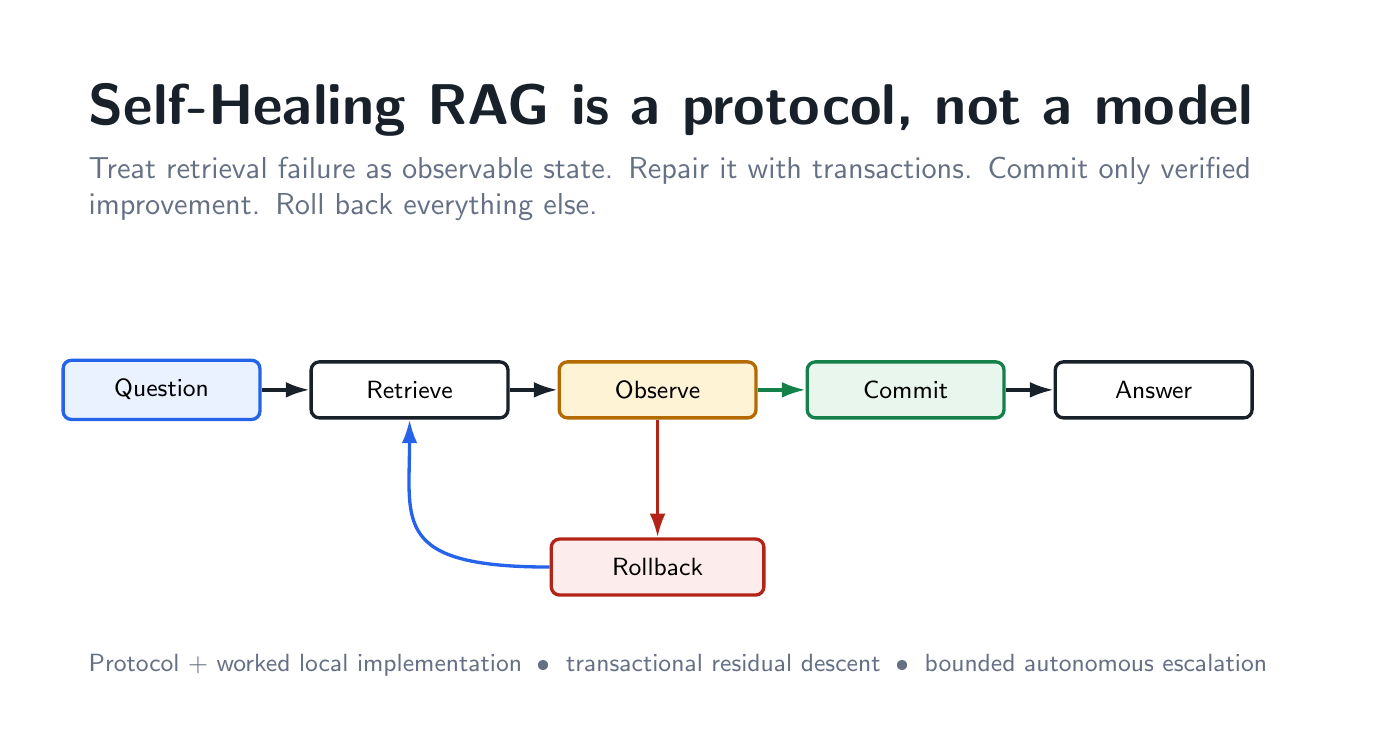
\begin{tikzpicture}
\fill[white] (-0.3,-0.4) rectangle (16.5,8.4);
\node[font=\sffamily\bfseries\fontsize{20}{24}\selectfont,text=ink,align=left,text width=158mm,anchor=west] at (0.35,7.35) {Self-Healing RAG is a protocol, not a model};
\node[font=\sffamily\fontsize{10.5}{13}\selectfont,text=gray,align=left,text width=154mm,anchor=west] at (0.35,6.35) {Treat retrieval failure as observable state. Repair it with transactions. Commit only verified improvement. Roll back everything else.};
\node[bluebox, minimum width=25mm] (q) at (1.4,3.8) {Question};
\node[box, minimum width=25mm] (r) at (4.55,3.8) {Retrieve};
\node[amberbox, minimum width=25mm] (o) at (7.7,3.8) {Observe};
\node[greenbox, minimum width=25mm] (c) at (10.85,3.8) {Commit};
\node[box, minimum width=25mm] (a) at (14.0,3.8) {Answer};
\draw[arrow] (q)--(r); \draw[arrow] (r)--(o); \draw[greenarrow] (o)--(c); \draw[arrow] (c)--(a);
\node[redbox, minimum width=27mm] (rb) at (7.7,1.55) {Rollback};
\draw[redarrow] (o)--(rb);
\draw[bluearrow] (rb.west) .. controls +(-20mm,0) and +(0,-13mm) .. (r.south);
\node[font=\sffamily\small,text=gray,align=left,text width=155mm,anchor=west] at (0.35,0.3) {Protocol + worked local implementation \;•\; transactional residual descent \;•\; bounded autonomous escalation};
\end{tikzpicture}
\end{document}
